 \chapter{Clustering}

%%%%%%%%%%%%%%%%%%%%%%%%%%%%%%%%%%%%%%%%%%%%%%%%%%%%%%%%%%%%%%%%%%%%%%%%%%%%%%%%%%%%%%%%%%
\section{K-means}
\subsection{Choice of attributes and distance function}

We have selected $3$ attributes to performe the clustering via the K-Means algorithm.
In particular we have ignored the categorical attributes as there isn't a proper metric to define a distance function over these kinds of attributes.

The used attributes are only: \textit{limit}, \textit{ba\_mean}, \textit{pa\_mean}. Note that we have excluded the age in this list as it is the only one that isn't measured in NTD.

For these attributes we used the euclidean distance as metric function as it is more natural for this kind of attributes.

\subsection{Choise of the best value of k}

To choose the best value of $k$ we have plotted for each $K$ between $2$ and $50$ the values of the SSE and the silhouette score. Each value is calculated as the best among $10$ runs (with the lowest SSE) and with a maximum of $300$ iterations of the K-Means algorithm.

\begin{figure}[h]
  \begin{minipage}[h]{.50\textwidth}
    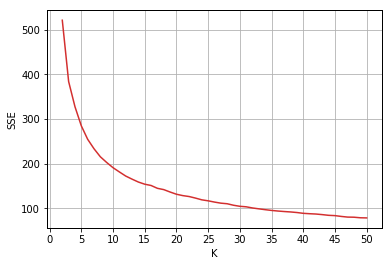
\includegraphics[width=1\textwidth]{img/ch3/kmeans_sse}
  \end{minipage}
    \begin{minipage}[h]{.50\textwidth}
    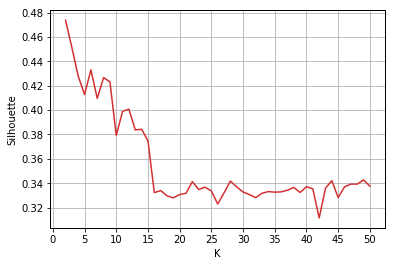
\includegraphics[width=1\textwidth]{img/ch3/kmeans_silhouette}
  \end{minipage}
\end{figure}

Using the elbow method we decide to set $k=6$ as it represents a good trade-off between SSE and data interpretability.

\subsection{Cluster analysis}

\begin{figure}[h]
  \begin{minipage}[h]{.40\textwidth}
    To better visualize the obtained clusters we have plotted the centers in parallel coordinates.
    
  From a first point of view we can see that all of the centers are separated in three class (low, medium, high) for all of the three used attributes.
  
  We want to go further in order to understand the different kind of customers and if there are some interesting correlation.
  \end{minipage}
    \begin{minipage}[h]{.60\textwidth}
    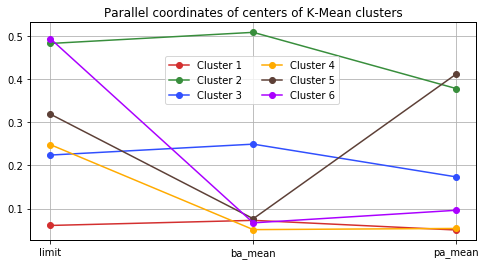
\includegraphics[width=1\textwidth]{img/ch3/kmeans_center}
  \end{minipage}
\end{figure}

\begin{figure}[h]
    \begin{minipage}[h]{.50\textwidth}
    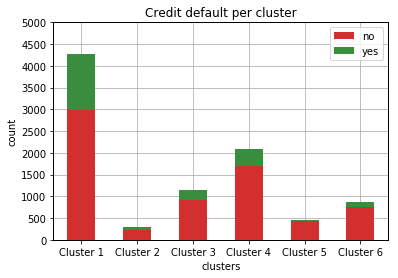
\includegraphics[width=1\textwidth]{img/ch3/kmeans_default}
  \end{minipage}
  \begin{minipage}[h]{.50\textwidth}
    
    We have also plotted the number of credit defaults for each cluster to trying to understand the distribution of the customers. The cluster with the most credit default is the first one, with a ratio of $30\%$ and the cluster with the lowest credit default is the fourth, with a ratio of $5\%$.
    
    Now we can pass to analyze each cluster individually.
      \end{minipage}
\end{figure}

\medskip

The \textcolor{red}{cluster 1} is the biggest, with $4276$ total elements include nearly half of the customers, and it is also the cluster with the highest credit default ratio. From the parallel coordinates plot we can see that the customers in this class have the credit cards with the lowest limit and also have the lowest bill/payment amounts over the six months.


The \textcolor{red}{cluster 2} bla bla.


The \textcolor{red}{cluster 3} bla bla.


The \textcolor{red}{cluster 4} bla bla.


The \textcolor{red}{cluster 5} bla bla.


The \textcolor{red}{cluster 6} bla bla.




\begin{figure}[h]
    \begin{minipage}[h]{.50\textwidth}
    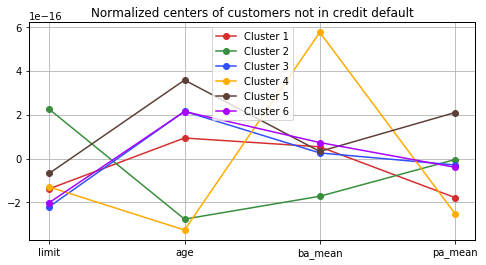
\includegraphics[width=1\textwidth]{img/ch3/kmeans_par_default_no}
  \end{minipage}
    \begin{minipage}[h]{.50\textwidth}
    
    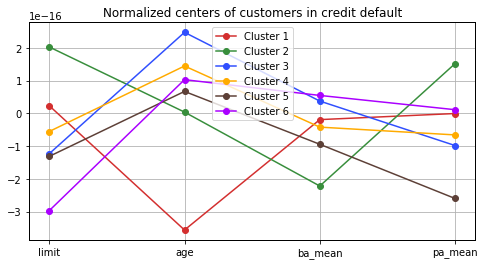
\includegraphics[width=1\textwidth]{img/ch3/kmeans_par_default_yes}
  \end{minipage}
\end{figure}


%%%%%%%%%%%%%%%%%%%%%%%%%%%%%%%%%%%%%%%%%%%%%%%%%%%%%%%%%%%%%%%%%%%%%%%%%%%%%%%%%%%%%%%%%%
\section{DBSCAN}
\subsection{Choice of attributes and distance function}
\subsection{Study of the clustering parameters}
\subsection{Characterization and interpretation of the obtained clusters}
%%%%%%%%%%%%%%%%%%%%%%%%%%%%%%%%%%%%%%%%%%%%%%%%%%%%%%%%%%%%%%%%%%%%%%%%%%%%%%%%%%%%%%%%%%
\section{Hierarchical clustering}
\subsection{Choice of attributes and distance function}
\subsection{Discussion of dendograms using different algorithms}
%%%%%%%%%%%%%%%%%%%%%%%%%%%%%%%%%%%%%%%%%%%%%%%%%%%%%%%%%%%%%%%%%%%%%%%%%%%%%%%%%%%%%%%%%%

\section{Evaluation of clustering approaches and comparison of the clustering obtained}
